\documentclass{beamer}
\usetheme{Madrid}
\usecolortheme{dolphin}
\usepackage{graphicx}
\usepackage{chemfig}
\usepackage{tikz}
\usepackage{amsmath}
\usepackage{mhchem}
\usepackage{listings}
\usepackage{lmodern}  % Latin Modern font package
\usepackage{pgfplots}  % For plotting charts
\pgfplotsset{compat=1.18}
\usepackage{amssymb}  % For checkmark symbol
\usepackage{pifont}  % For cross mark symbol
\usepackage{ragged2e}  % For proper column alignment in beamer
\usetikzlibrary{shapes,arrows,positioning,fit,backgrounds}
\definecolor{mygreen}{RGB}{28,172,0}
\definecolor{mylilas}{RGB}{170,55,241}
\definecolor{mygray}{RGB}{128,128,128}
% Professional color palette for MIT/Stanford-quality slides
\definecolor{primary}{RGB}{0,51,102}      % Deep blue
\definecolor{secondary}{RGB}{204,85,0}    % Burnt orange
\definecolor{accent1}{RGB}{0,136,55}      % Forest green
\definecolor{neutral}{RGB}{128,128,128}   % Gray
\definecolor{highlight}{RGB}{255,204,0}   % Gold
\definecolor{warning}{RGB}{204,85,0}      % Warning color (orange/red)



\lstset{
  language=Python,
  basicstyle=\ttfamily\footnotesize,
  keywordstyle=\color{blue}\bfseries,
  commentstyle=\color{gray}\itshape,
  stringstyle=\color{orange},
  numberstyle=\tiny\color{gray},
  showstringspaces=false,
  breaklines=true,
  frame=single,
  framesep=3pt,
  framexleftmargin=3pt,
  backgroundcolor=\color{blue!5},
  rulecolor=\color{blue!30},
  xleftmargin=5pt,
  xrightmargin=5pt,
  aboveskip=8pt,
  belowskip=8pt,
}

% Set Latin Modern Roman as default font
\renewcommand{\rmdefault}{lmr}
\renewcommand{\sfdefault}{lmr}  % Override Beamer's default sans-serif with lmr
\renewcommand{\ttdefault}{lmtt}
% Force text to use roman font instead of sans-serif
\usefonttheme{professionalfonts}
\setbeamerfont{normal text}{family=\rmfamily}


% Modify navigation bar to only show sections (outline)
\beamertemplatenavigationsymbolsempty  % Remove navigation symbols
\setbeamertemplate{footline}{}  % Remove the footer completely

\title{An Introduction to Graph Neural Networks (GNNs) for Molecules}
\author{MPS6 Course}
\date{10.04.2025}
%%%%%%%%%%%%%%%%%%%%%%%%%%%%%%%%%%%%%%%%%%%%%%%%%%%%%%%%%%%%%%%%
\begin{document}

\begin{frame}
    \titlepage
\end{frame}

\begin{frame}{Course Outline}
    \begin{itemize}
        \item What is a graph?
        \item Representing molecules as graphs
        \item Different tasks with GNNs
        \item Message passing on molecular graphs
        \item Introduction to PyTorch Geometric
        \item Developing a GCN from scratch
        \item Hands-on implementation
    \end{itemize}
\end{frame}
%%%%%%%%%%%%%%%%%%%%%%%%%%%%%%%%%%%%%%%%%%%%%%%%%%%%%%%%%%%%%%%%%
% Section: What is a graph?
\section{What is a Graph?}

\begin{frame}{What is a Graph?}
    \begin{columns}
        \begin{column}{0.7\textwidth}
            \begin{itemize}
                \item A graph $G = (V, E)$ consists of:
                \begin{itemize}
                    \item Nodes/vertices $V$
                    \item Edges $E$ connecting nodes
                \end{itemize}
                \item Graphs represent relational data
                \item Natural representation for molecules
            \end{itemize}
        \end{column}
        \begin{column}{0.3\textwidth}
            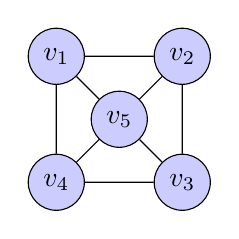
\begin{tikzpicture}[scale=0.8]
                \node[circle, draw, fill=blue!20] (A) at (0,2) {$v_1$};
                \node[circle, draw, fill=blue!20] (B) at (2,2) {$v_2$};
                \node[circle, draw, fill=blue!20] (C) at (2,0) {$v_3$};
                \node[circle, draw, fill=blue!20] (D) at (0,0) {$v_4$};
                \node[circle, draw, fill=blue!20] (E) at (1,1) {$v_5$};
                
                \draw (A) -- (B) -- (C) -- (D) -- (A);
                \draw (A) -- (E) -- (B);
                \draw (C) -- (E) -- (D);
            \end{tikzpicture}
        \end{column}
    \end{columns}
\end{frame}
%%%%%%%%%%%%%%%%%%%%%%%%%%%%%%%%%%%%%%%%%%%%%%%%%%%%%%%%%%%%%%%%%%%%

\begin{frame}{Adjacency Matrix}
    \begin{columns}
        \begin{column}{0.4\textwidth}
            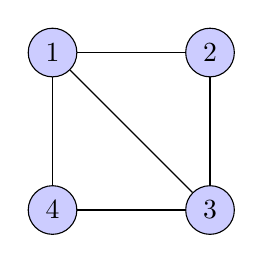
\begin{tikzpicture}[scale=1.0]
                \node[circle, draw, fill=blue!20] (1) at (0,2) {$1$};
                \node[circle, draw, fill=blue!20] (2) at (2,2) {$2$};
                \node[circle, draw, fill=blue!20] (3) at (2,0) {$3$};
                \node[circle, draw, fill=blue!20] (4) at (0,0) {$4$};
                
                \draw (1) -- (2) -- (3) -- (4) -- (1);
                \draw (1) -- (3);
            \end{tikzpicture}
        \end{column}
        \begin{column}{0.6\textwidth}
            Adjacency matrix $A \in \{0,1\}^{n \times n}$:
            
            \[
            A = \begin{pmatrix}
            0 & 1 & 1 & 1 \\
            1 & 0 & 1 & 0 \\
            1 & 1 & 0 & 1 \\
            1 & 0 & 1 & 0
            \end{pmatrix}
            \]
            
            \begin{itemize}
                \item $A_{ij} = 1$ if nodes $i$ and $j$ are connected
                \item $A_{ij} = 0$ otherwise
                \item Can also have weighted edges where $A_{ij} \in \mathbb{R}$
            \end{itemize}
        \end{column}
    \end{columns}
\end{frame}
%%%%%%%%%%%%%%%%%%%%%%%%%%%%%%%%%%%%%%%%%%%%%%%%%%%%%%%%%%%%%%%%%%

\begin{frame}{Node and Edge Features}
    \begin{columns}
        \begin{column}{0.6\textwidth}
            \textbf{Node Features}:
            \begin{itemize}
                \item Each node $v_i$ has features $\mathbf{x}_i$
                \item Can be categorical or continuous
                \item For molecules: atom type, charge, hybridization, etc.
            \end{itemize}
            
            \textbf{Edge Features}:
            \begin{itemize}
                \item Each edge $(v_i, v_j)$ has features $\mathbf{e}_{ij}$
                \item For molecules: bond type, distance, etc.
            \end{itemize}
        \end{column}
        \begin{column}{0.4\textwidth}
            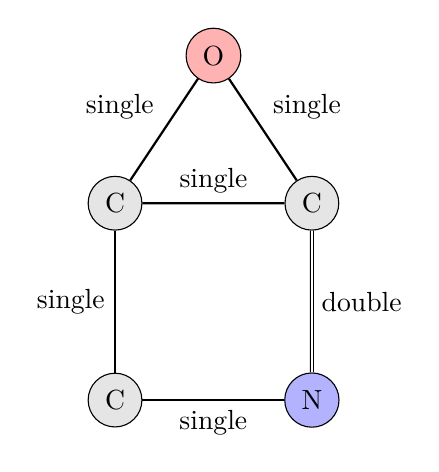
\begin{tikzpicture}[scale=1.25]
                \node[circle, draw, fill=gray!20] (A) at (0,2) {C};
                \node[circle, draw, fill=gray!20] (B) at (2,2) {C};
                \node[circle, draw, fill=blue!30] (C) at (2,0) {N};
                \node[circle, draw, fill=gray!20] (D) at (0,0) {C};
                \node[circle, draw, fill=red!30] (E) at (1,3.5) {O};
                
                \draw[thick] (A) -- node[above] {single} (B);
                \draw[double] (B) -- node[right] {double} (C);
                \draw[thick] (C) -- node[below] {single} (D);
                \draw[thick] (D) -- node[left] {single} (A);
                \draw[thick] (A) -- node[above left] {single} (E);
                \draw[thick] (B) -- node[above right] {single} (E);
            \end{tikzpicture}
        \end{column}
    \end{columns}
\end{frame}
%%%%%%%%%%%%%%%%%%%%%%%%%%%%%%%%%%%%%%%%%%%%%%%%%%%%%%%%%%%%%%%%%%%%%
% Section: Representing a Molecule as a Graph
\section{Representing a Molecule as a Graph}

\begin{frame}{Representing a Molecule as a Graph}
    \begin{columns}
        \begin{column}{0.5\textwidth}
            \begin{itemize}
                \item Nodes = Atoms
                \item Edges = Bonds
                \item Node features = Atom properties
                \item Edge features = Bond properties
            \end{itemize}
        \end{column}
        \begin{column}{0.5\textwidth}
            \begin{center}
                \chemfig{CH_3-CH_2-OH}
                
                \vspace{0.5cm}
                
                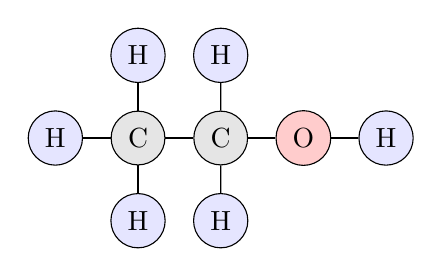
\begin{tikzpicture}[scale=0.7]
                    \node[circle, draw, fill=gray!20] (C1) at (0,0) {C};
                    \node[circle, draw, fill=gray!20] (C2) at (1.5,0) {C};
                    \node[circle, draw, fill=red!20] (O) at (3,0) {O};
                    \node[circle, draw, fill=blue!10] (H1) at (0,1.5) {H};
                    \node[circle, draw, fill=blue!10] (H2) at (0,-1.5) {H};
                    \node[circle, draw, fill=blue!10] (H3) at (-1.5,0) {H};
                    \node[circle, draw, fill=blue!10] (H4) at (1.5,1.5) {H};
                    \node[circle, draw, fill=blue!10] (H5) at (1.5,-1.5) {H};
                    \node[circle, draw, fill=blue!10] (H6) at (4.5,0) {H};
                    
                    \draw (C1) -- (C2) -- (O) -- (H6);
                    \draw (C1) -- (H1);
                    \draw (C1) -- (H2);
                    \draw (C1) -- (H3);
                    \draw (C2) -- (H4);
                    \draw (C2) -- (H5);
                \end{tikzpicture}
            \end{center}
        \end{column}
    \end{columns}
\end{frame}
%%%%%%%%%%%%%%%%%%%%%%%%%%%%%%%%%%%%%%%%%%%%%%%%%%%%%%%%%%%%%%%%%%%%%%%%%%%%
\begin{frame}{Node Features for Molecules}
    Common atom (node) features:
    
    \begin{itemize}
        \item Atomic number (one-hot or embedding)
        \item Atom type (C, H, O, N, etc.)
        \item Formal charge
        \item Hybridization state (sp, sp$^2$, sp$^3$)
        \item Number of hydrogens attached
        \item Is in aromatic ring?
        \item Chirality
        \item Partial charge
    \end{itemize}
    
    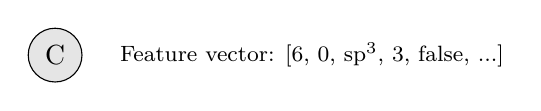
\begin{tikzpicture}[scale=0.7]
        \node[circle, draw, fill=gray!20] (C) at (0,0) {\ce{C}};
        \node[right] at (1,0) {\footnotesize Feature vector: [6, 0, sp$^3$, 3, false, ...]};
    \end{tikzpicture}
\end{frame}

\begin{frame}{Edge Features for Molecules}
    Common bond (edge) features:
    
    \begin{itemize}
        \item Bond type (single, double, triple, aromatic)
        \item Bond distance
        \item Is in ring?
        \item Conjugation
        \item Stereochemistry (cis/trans)
    \end{itemize}
    
    \begin{center}
        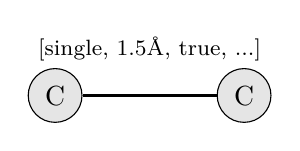
\begin{tikzpicture}[scale=0.8]
            \node[circle, draw, fill=gray!20] (C1) at (0,0) {C};
            \node[circle, draw, fill=gray!20] (C2) at (3,0) {C};
            
            \draw[thick] (C1) -- node[above=0.3cm] {\footnotesize [single, 1.5Å, true, ...]} (C2);
        \end{tikzpicture}
        
        \vspace{0.5cm}
        
        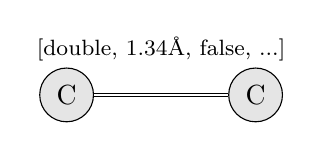
\begin{tikzpicture}[scale=0.8]
            \node[circle, draw, fill=gray!20] (C1) at (0,0) {C};
            \node[circle, draw, fill=gray!20] (C2) at (3,0) {C};
            
            \draw[double] (C1) -- node[above=0.3cm] {\footnotesize [double, 1.34Å, false, ...]} (C2);
        \end{tikzpicture}
    \end{center}
\end{frame}
%%%%%%%%%%%%%%%%%%%%%%%%%%%%%%%%%%%%%%%%%%%%%%%%%%%%%%%%%%%%%%%%%%%%%%%%
\begin{frame}{Methanol Example}
    \begin{columns}
        \begin{column}{0.45\textwidth}
            \textbf{Methanol (CH$_3$OH)}
            
            \vspace{0.3cm}
            
            \begin{center}
                \chemfig{CH_3-OH}
            \end{center}
            
            \vspace{0.3cm}
            
            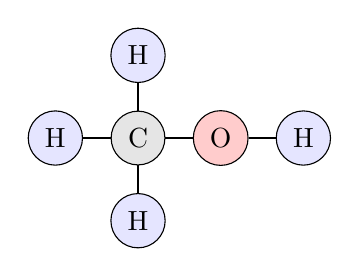
\begin{tikzpicture}[scale=0.7]
                \node[circle, draw, fill=gray!20] (C) at (0,0) {C};
                \node[circle, draw, fill=red!20] (O) at (1.5,0) {O};
                \node[circle, draw, fill=blue!10] (H1) at (0,1.5) {H};
                \node[circle, draw, fill=blue!10] (H2) at (-1.5,0.0) {H};
                \node[circle, draw, fill=blue!10] (H3) at (0,-1.5) {H};
                \node[circle, draw, fill=blue!10] (H4) at (3.0,0) {H};
                
                \draw (C) -- (O) -- (H4);
                \draw (C) -- (H1);
                \draw (C) -- (H2);
                \draw (C) -- (H3);
            \end{tikzpicture}
        \end{column}
        \begin{column}{0.55\textwidth}
            \textbf{Graph Representation:}
            
            \textbf{Nodes:}
            \begin{itemize}
                \item C: [6, 0, sp$^3$, 3, 0]
                \item O: [8, 0, sp$^3$, 1, 0]
                \item H$_1$-H$_4$: [1, 0, s, 0, 0]
            \end{itemize}
            
            \textbf{Adjacency Matrix:}
            {\tiny
            \[
            A = \begin{pmatrix}
            0 & 1 & 1 & 1 & 1 & 0 \\
            1 & 0 & 0 & 0 & 0 & 1 \\
            1 & 0 & 0 & 0 & 0 & 0 \\
            1 & 0 & 0 & 0 & 0 & 0 \\
            1 & 0 & 0 & 0 & 0 & 0 \\
            0 & 1 & 0 & 0 & 0 & 0
            \end{pmatrix}
            \]
            }
            
            \textbf{Node ordering:} C, O, H$_1$, H$_2$, H$_3$, H$_4$
        \end{column}
    \end{columns}
\end{frame}
%%%%%%%%%%%%%%%%%%%%%%%%%%%%%%%%%%%%%%%%%%%%%%%%%%%%%%%%%%%%%%%%%%%%%%%%%%%%
\begin{frame}{Real-World Molecular Features}
    \textbf{Node Features} (21 dimensions per atom in practice):
    \vspace{0.5cm}
    
    \begin{columns}
        \begin{column}{0.8\textwidth}
            \centering
            \small
            \begin{tabular}{ll}
                \hline
                \textbf{Feature Group} & \textbf{Dimensions} \\
                \hline
                Atom type (one-hot) & 11 \\
                \footnotesize (C, O, N, H, F, P, S, Cl, Br, I, Other) & \\
                Formal charge & 1 \\
                Aromaticity & 1 \\
                Ring membership & 1 \\
                Degree (number of bonds) & 1 \\
                Total hydrogens & 1 \\
                Radical electrons & 1 \\
                Hybridization (one-hot) & 4 \\
                \footnotesize (sp, sp$^2$, sp$^3$, Other) & \\
                \hline
                \textbf{Total} & \textbf{21} \\
                \hline
            \end{tabular}
        \end{column}
    \end{columns}
\end{frame}

%%%%%%%%%%%%%%%%%%%%%%%%%%%%%%%%%%%%%%%%%%%%%%%%%%%%%%%%%%%%%%%%%%%%%%%%%%%%
\begin{frame}{Real-World Molecular Features}
    \textbf{Edge Features} (6 dimensions per bond in practice):
    \begin{columns}
        \begin{column}{0.8\textwidth}
            \begin{itemize}
                \item Bond type (one-hot, 4D)
                \begin{itemize}
                    \footnotesize
                    \item Single, double, triple, aromatic
                \end{itemize}
                \item Conjugation (1D)
                \item Ring membership (1D)
            \end{itemize}

            \vspace{0.5cm}

            \textbf{Why this matters:}
            \begin{itemize}
                \footnotesize
                \item Chemical significance drives feature choice
                \item More features = better predictions
                \item But: curse of dimensionality
            \end{itemize}
        \end{column}
    \end{columns}
\end{frame}
%%%%%%%%%%%%%%%%%%%%%%%%%%%%%%%%%%%%%%%%%%%%%%%%%%%%%%%%%%%%%%%%%%%%%%%%%%%%
\begin{frame}{Hands-On Session}
\begin{center}
\begin{tikzpicture}
\node[rectangle, rounded corners, fill=blue!10, minimum width=8cm, minimum height=1.5cm, text width=7.5cm, align=center] at (0,2) {\Large Let's put theory into practice!};
        \node[rectangle, draw=none, text width=7.5cm, align=left] at (0,-2) {
            \begin{itemize}
                \item Open your Python notebook
                \item We'll learn how to represent graph in Python
                \item We'll learn graph representation in PyTorch Geometric
                \item Resources: \url{https://github.com/HFooladi/GNNs-For-Chemists/blob/main/notebooks/01_GNN_representation.ipynb}
            \end{itemize}
        };
\end{tikzpicture}
\end{center}
\end{frame}
%%%%%%%%%%%%%%%%%%%%%%%%%%%%%%%%%%%%%%%%%%%%%%%%%%%%%%%%%%%%%%%%%%%%%%%%%%%%%
% Section: GNN Tasks
\section{GNN Tasks for Molecules}

\begin{frame}{Different Tasks with Graph Neural Networks}
    \begin{columns}
        \begin{column}{0.5\textwidth}
            \textbf{Node-level tasks:}
            \begin{itemize}
                \item Atom property prediction
                \item Reaction site prediction
                \item Partial charge prediction
            \end{itemize}
            
            \textbf{Edge-level tasks:}
            \begin{itemize}
                \item Bond property prediction
                \item Link prediction (e.g., potential bonds)
            \end{itemize}
        \end{column}
        \begin{column}{0.5\textwidth}
            \textbf{Graph-level tasks:}
            \begin{itemize}
                \item Molecular property prediction
                \begin{itemize}
                    \item Solubility
                    \item Toxicity
                    \item Drug efficacy
                    \item Binding affinity
                \end{itemize}
                \item Molecule generation
                \item Molecule classification
            \end{itemize}
        \end{column}
    \end{columns}
    
    \vspace{0.5cm}
    
    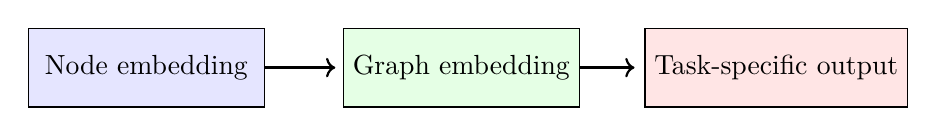
\begin{tikzpicture}
        \node[rectangle, draw, fill=blue!10, minimum width=3cm, minimum height=1cm] at (0,0) {Node embedding};
        \node[rectangle, draw, fill=green!10, minimum width=3cm, minimum height=1cm] at (4,0) {Graph embedding};
        \node[rectangle, draw, fill=red!10, minimum width=3cm, minimum height=1cm] at (8,0) {Task-specific output};
        
        \draw[->, thick] (1.5,0) -- (2.4,0);
        \draw[->, thick] (5.5,0) -- (6.2,0);
    \end{tikzpicture}
\end{frame}
%%%%%%%%%%%%%%%%%%%%%%%%%%%%%%%%%%%%%%%%%%%%%%%%%%%%%%%%%%%%%%%%%%%%%%%%%%%%%
\begin{frame}{Graph-Level Property Prediction}
    \begin{center}
        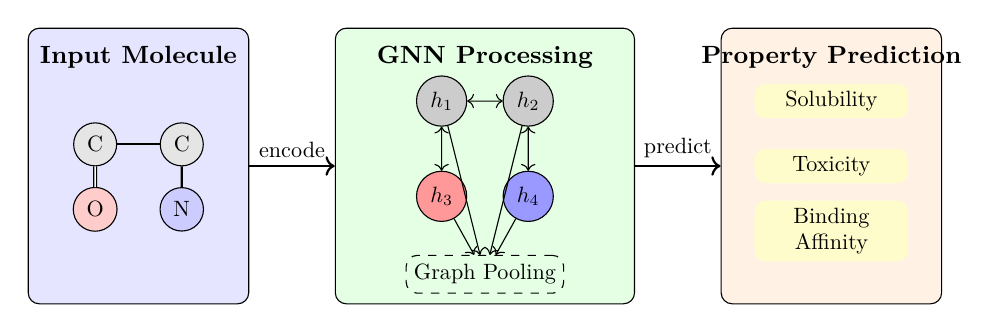
\begin{tikzpicture}[scale=0.55]
            % Input molecule (left side)
            \node[rectangle, draw, rounded corners, fill=blue!10, minimum width=2.8cm, minimum height=3.5cm] (molecule) at (-8,0) {};
            \node at (-8,2.5) {\small\textbf{Input Molecule}};
            
            % Draw molecule structure inside the box
            \node[circle, draw, fill=gray!20, scale=0.8] (C1) at (-9,0.5) {C};
            \node[circle, draw, fill=gray!20, scale=0.8] (C2) at (-7,0.5) {C};
            \node[circle, draw, fill=red!20, scale=0.8] (O) at (-9,-1.0) {O};
            \node[circle, draw, fill=blue!20, scale=0.8] (N) at (-7,-1.0) {N};
            
            \draw[thick] (C1) -- (C2);
            \draw[double] (C1) -- (O);
            \draw[thick] (C2) -- (N);
            
            % GNN processing (middle)
            \node[rectangle, draw, rounded corners, fill=green!10, minimum width=3.8cm, minimum height=3.5cm] (gnn) at (0,0) {};
            \node at (0,2.5) {\small\textbf{GNN Processing}};
            
            % Draw GNN internals
            \node[circle, draw, fill=gray!40, minimum size=0.7cm, scale=0.8] (n1) at (-1,1.5) {$h_1$};
            \node[circle, draw, fill=gray!40, minimum size=0.7cm, scale=0.8] (n2) at (1,1.5) {$h_2$};
            \node[circle, draw, fill=red!40, minimum size=0.7cm, scale=0.8] (n3) at (-1,-0.7) {$h_3$};
            \node[circle, draw, fill=blue!40, minimum size=0.7cm, scale=0.8] (n4) at (1,-0.7) {$h_4$};
            
            \draw[<->] (n1) -- (n2);
            \draw[<->] (n1) -- (n3);
            \draw[<->] (n2) -- (n4);
            
            \node[rectangle, draw, dashed, rounded corners, minimum width=2.5cm, minimum height=0.6cm, scale=0.8] (pool) at (0,-2.5) {Graph Pooling};
            
            \draw[->] (n1) -- (pool);
            \draw[->] (n2) -- (pool);
            \draw[->] (n3) -- (pool);
            \draw[->] (n4) -- (pool);
            
            % Property prediction (right side)
            \node[rectangle, draw, rounded corners, fill=orange!10, minimum width=2.8cm, minimum height=3.5cm] (prediction) at (8,0) {};
            \node at (8,2.5) {\small\textbf{Property Prediction}};
            
            % Example properties - more compact
            \node[rectangle, fill=yellow!20, rounded corners, minimum width=2.2cm, text width=2.2cm, align=center, scale=0.8] at (8,1.5) {Solubility};
            \node[rectangle, fill=yellow!20, rounded corners, minimum width=2.2cm, text width=2.2cm, align=center, scale=0.8] at (8,0.0) {Toxicity};
            \node[rectangle, fill=yellow!20, rounded corners, minimum width=2.2cm, text width=2.2cm, align=center, scale=0.8] at (8,-1.5) {Binding Affinity};
            
            % Flow arrows
            \draw[->, thick] (molecule) -- (gnn) node[midway, above, scale=0.8] {encode};
            \draw[->, thick] (gnn) -- (prediction) node[midway, above, scale=0.8] {predict};
        \end{tikzpicture}
    \end{center}
    
    \vspace{0.1cm}
    
    \begin{columns}
        \begin{column}{0.48\textwidth}
            \textbf{Process:}
            \begin{itemize}
                \item Encode molecular structure
                \item Message passing between atoms
                \item Pool features → molecule representation
                \item Predict properties
            \end{itemize}
        \end{column}
        \begin{column}{0.52\textwidth}
            \textbf{Applications:}
            \begin{itemize}
                \item Binding affinity prediction
                \item Virtual screening
                \item Toxicity screening
                \item Reaction yield prediction
            \end{itemize}
        \end{column}
    \end{columns}
\end{frame}
%%%%%%%%%%%%%%%%%%%%%%%%%%%%%%%%%%%%%%%%%%%%%%%%%%%%%%%%%%%%%%%%%%%%%%%%%%%%
% Section: Message passing on molecular graphs
\section{Message passing on molecular graphs}
\begin{frame}{Message Passing Neural Networks}
    \begin{columns}
        \begin{column}{0.55\textwidth}
            \textbf{Message Passing Framework:}
            \begin{enumerate}
                \item Each node sends messages to its neighbors
                \item Each node aggregates incoming messages
                \item Each node updates its features based on aggregated messages
            \end{enumerate}
            
            \vspace{0.3cm}
            
            \textbf{Mathematical formulation:}
            \begin{align}
            m_{i}^{(l+1)} &= \sum_{j \in \mathcal{N}(i)} M(h_i^{(l)}, h_j^{(l)}, e_{ij}) \\
            h_i^{(l+1)} &= U(h_i^{(l)}, m_{i}^{(l+1)})
            \end{align}
            
            where $M$ is the message function and $U$ is the update function.
        \end{column}
        \begin{column}{0.45\textwidth}
            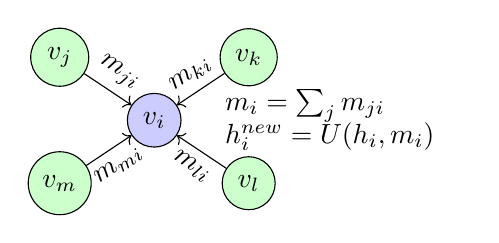
\begin{tikzpicture}[scale=0.8]
                % Central node
                \node[circle, draw, fill=blue!20] (A) at (0,0) {$v_i$};
                
                % Neighbor nodes
                \node[circle, draw, fill=green!20] (B) at (-1.5,1) {$v_j$};
                \node[circle, draw, fill=green!20] (C) at (1.5,1) {$v_k$};
                \node[circle, draw, fill=green!20] (D) at (1.5,-1) {$v_l$};
                \node[circle, draw, fill=green!20] (E) at (-1.5,-1) {$v_m$};
                
                % Connect nodes
                \draw[->] (B) -- node[above, sloped] {$m_{ji}$} (A);
                \draw[->] (C) -- node[above, sloped] {$m_{ki}$} (A);
                \draw[->] (D) -- node[below, sloped] {$m_{li}$} (A);
                \draw[->] (E) -- node[below, sloped] {$m_{mi}$} (A);
                
                % Aggregation
                \node[text width=3cm] at (3,0) {$m_i = \sum_j m_{ji}$\\$h_i^{new} = U(h_i, m_i)$};
            \end{tikzpicture}
            
            \vspace{0.5cm}
            
            Message passing allows the model to:
            \begin{itemize}
                \item Capture local chemical environment
                \item Learn hierarchical representations
                \item Handle molecules of different sizes
            \end{itemize}
        \end{column}
    \end{columns}
\end{frame}
%%%%%%%%%%%%%%%%%%%%%%%%%%%%%%%%%%%%%%%%%%%%%%%%%%%%%%%%%%%%%%%%%%%%%%%%%%%%%
\begin{frame}{What is Equivariance?}
    \begin{columns}
        \begin{column}{0.6\textwidth}
            \textbf{Equivariance} means that transformations of input lead to predictable transformations of output.
            
            \vspace{0.3cm}
            
            For molecules:
            \begin{itemize}
                \item Rotation/translation of a molecule shouldn't change its properties
                \item Permutation equivariance
            \end{itemize}
            
            \vspace{0.3cm}
            
            Why it matters:
            \begin{itemize}
                \item Ensures consistent predictions regardless of orientation
                \item Reduces required training data
                \item More physically meaningful representations
            \end{itemize}
        \end{column}
        \begin{column}{0.4\textwidth}
            \begin{center}
                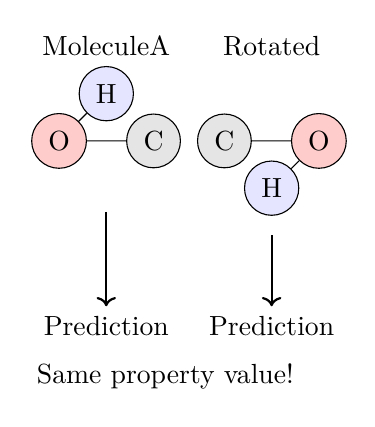
\begin{tikzpicture}[scale=0.6]
                    % Original molecule
                    \node[circle, draw, fill=red!20] (O1) at (0,0) {O};
                    \node[circle, draw, fill=gray!20] (C1) at (2,0) {C};
                    \node[circle, draw, fill=blue!10] (H1) at (1,1) {H};
                    
                    \draw (C1) -- (O1) -- (H1);
                    
                    \node at (1.0,2) {MoleculeA};
                    
                    % Rotated molecule
                    \node[circle, draw, fill=gray!20] (C2) at (3.5,0) {C};
                    \node[circle, draw, fill=red!20] (O2) at (5.5,0) {O};
                    \node[circle, draw, fill=blue!10] (H2) at (4.5,-1) {H};
                    
                    \draw (C2) -- (O2) -- (H2);
                    
                    \node at (4.5,2) {Rotated};
                    
                    % Same prediction arrow
                    \draw[->, thick] (1.0,-1.5) -- (1.0,-3.5) node[below] {Prediction};
                    \draw[->, thick] (4.5,-2.0) -- (4.5,-3.5) node[below] {Prediction};
                    
                    \node at (2.25,-5) {Same property value!};
                \end{tikzpicture}
            \end{center}
        \end{column}
    \end{columns}
\end{frame}
%%%%%%%%%%%%%%%%%%%%%%%%%%%%%%%%%%%%%%%%%%%%%%%%%%%%%%%%%%%%%%%%%%%%%%%%%%%%%%%%%%%
\begin{frame}{Permutation Equivariance in GNNs}
\begin{columns}
\begin{column}{0.45\textwidth}
\textbf{Permutation Equivariance:}
\begin{itemize}
\item Reordering nodes before applying a GNN should give the same result as applying the GNN first and then reordering nodes
\item Critical for molecules where node ordering is arbitrary
\end{itemize}
        \vspace{0.1cm}
        \small{Mathematically: for a GNN function $f$ and permutation $P$:
        \[ f(PX, PAP^T) = Pf(X, A) \]}
    \end{column}
    \begin{column}{0.55\textwidth}
        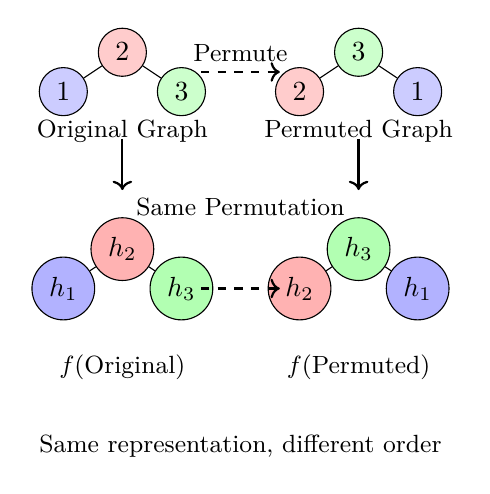
\begin{tikzpicture}[scale=0.5]
            % Original graph (top left)
            \node[circle, draw, fill=blue!20] (A1) at (0,5) {1};
            \node[circle, draw, fill=red!20] (B1) at (1.5,6) {2};
            \node[circle, draw, fill=green!20] (C1) at (3,5) {3};
            
            \draw (A1) -- (B1) -- (C1);
            \node at (1.5,4) {\small Original Graph};
            
            % Permuted graph (top right)
            \node[circle, draw, fill=red!20] (B2) at (6,5) {2};
            \node[circle, draw, fill=green!20] (C2) at (7.5,6) {3};
            \node[circle, draw, fill=blue!20] (A2) at (9,5) {1};
            
            \draw (B2) -- (C2) -- (A2);
            \node at (7.5,4) {\small Permuted Graph};
            
            % Result 1 (bottom left)
            \node[circle, draw, fill=blue!30] (A3) at (0,0) {$h_1$};
            \node[circle, draw, fill=red!30] (B3) at (1.5,1) {$h_2$};
            \node[circle, draw, fill=green!30] (C3) at (3,0) {$h_3$};
            
            \draw (A3) -- (B3) -- (C3);
            \node at (1.5,-2) {\small $f($Original$)$};
            
            % Result 2 (bottom right)
            \node[circle, draw, fill=red!30] (B4) at (6,0) {$h_2$};
            \node[circle, draw, fill=green!30] (C4) at (7.5,1) {$h_3$};
            \node[circle, draw, fill=blue!30] (A4) at (9,0) {$h_1$};
            
            \draw (B4) -- (C4) -- (A4);
            \node at (7.5,-2) {\small $f($Permuted$)$};
            
            % Arrows
            \draw[->, thick] (1.5,3.8) -- (1.5,2.5);
            \draw[->, thick] (7.5,3.8) -- (7.5,2.5);
            
            % Permutation arrows
            \draw[->, thick, dashed] (3.5,5.5) -- (5.5,5.5) node[midway, above] {\small Permute};
            \draw[->, thick, dashed] (3.5,0) -- (5.5,0) node[midway, above=0.8cm] {\small Same Permutation};
            
            % Equal sign
            \node at (4.5,-4) {\small Same representation, different order};
        \end{tikzpicture}
    \end{column}
\end{columns}
\end{frame}
%%%%%%%%%%%%%%%%%%%%%%%%%%%%%%%%%%%%%%%%%%%%%%%%%%%%%%%%%%%%%%%%%%%%%%%%%%%%%%%%%%%%%%%
\begin{frame}{Hands-On Session}
\begin{center}
\begin{tikzpicture}
\node[rectangle, rounded corners, fill=blue!10, minimum width=8cm, minimum height=1.5cm, text width=7.5cm, align=center] at (0,2) {\Large Let's put theory into practice!};
        \node[rectangle, draw=none, text width=7.5cm, align=left] at (0,-2) {
            \begin{itemize}
                \item Open your Python notebook
                \item We'll learn how to implement message passing
                \item Resources: \url{https://github.com/HFooladi/GNNs-For-Chemists/blob/main/notebooks/02_GNN_message_passing.ipynb}
            \end{itemize}
        };
\end{tikzpicture}
\end{center}
\end{frame}

%%%%%%%%%%%%%%%%%%%%%%%%%%%%%%%%%%%%%%%%%%%%%%%%%%%%%%%%%%%%%%%%%%%%%%%%%%%%%%%%%%%%%%%%%5
% Section: PyTorch Geometric
\section{Introduction to PyTorch Geometric}

\begin{frame}[fragile]{Introduction to PyTorch Geometric (PyG)}
    \begin{itemize}
        \item PyTorch Geometric (PyG) is a library for deep learning on irregular structures (graphs, point-clouds, etc.)
        \item Built on top of PyTorch
        \item Provides tools for working with graphs
        \item Efficient implementations of many GNN architectures
    \end{itemize}
    
    \begin{lstlisting}[language=Python]
    # Installing PyTorch Geometric
    pip install torch-geometric
    
    # Basic imports
    import torch
    from torch_geometric.data import Data
    from torch_geometric.nn import GCNConv
    \end{lstlisting}
\end{frame}

\begin{frame}[fragile]{Downloading and Loading Datasets}
    \begin{lstlisting}[language=Python, basicstyle=\ttfamily\scriptsize]
from torch_geometric.datasets import MoleculeNet

# Download BACE dataset (biological activity prediction)
dataset = MoleculeNet(root='data/molecule_datasets', name='BACE')

print(f'Dataset size: {len(dataset)}')
print(f'Number of features: {dataset.num_features}')

# Look at the first graph
data = dataset[0]

# Splitting into train, validation, test
from torch_geometric.loader import DataLoader
from sklearn.model_selection import train_test_split

train_idx, test_idx = train_test_split(
    range(len(dataset)), test_size=0.2, random_state=42)
train_idx, val_idx = train_test_split(
    train_idx, test_size=0.25, random_state=42)
    \end{lstlisting}
\end{frame}

\begin{frame}[fragile]{Exploring the Dataset Features}
    \begin{lstlisting}[language=Python, basicstyle=\ttfamily\scriptsize]
# Explore a single molecule
data = dataset[0]
print("Node features shape:", data.x.shape)
print("Edge indices shape:", data.edge_index.shape)

# Visualize the molecule
from rdkit import Chem
from rdkit.Chem import Draw

smiles = data.smiles
mol = Chem.MolFromSmiles(smiles)
img = Draw.MolToImage(mol, size=(300, 300))
plt.imshow(img)
plt.axis('off')

# Analyzing feature distributions
node_features = []
for data in dataset[:100]:
    node_features.append(data.x.mean(dim=0))
average_features = torch.stack(node_features).mean(dim=0)
plt.bar(range(len(average_features)), average_features.numpy())
    \end{lstlisting}
\end{frame}
%%%%%%%%%%%%%%%%%%%%%%%%%%%%%%%%%%%%%%%%%%%%%%%%%%%%%%%%%%%%%%%%%%%%%%%%%%%%%%%%%%%%%%%%%%%%5
% Section: Developing a GCN
\section{Developing a GCN from Scratch}

\begin{frame}{Graph Convolutional Network (GCN) Layer}
    \begin{columns}
        \begin{column}{0.6\textwidth}
            GCN update rule:
            \begin{align}
            H^{(l+1)} = \sigma(\tilde{D}^{-\frac{1}{2}}\tilde{A}\tilde{D}^{-\frac{1}{2}}H^{(l)}W^{(l)})
            \end{align}
            
            where:
            \begin{itemize}
                \item $\tilde{A} = A + I$ (adjacency matrix with self-loops)
                \item $\tilde{D}$ is the degree matrix of $\tilde{A}$
                \item $H^{(l)}$ is the node feature matrix at layer $l$
                \item $W^{(l)}$ is the learnable weight matrix
                \item $\sigma$ is a non-linear activation function
            \end{itemize}
        \end{column}
        \begin{column}{0.4\textwidth}
            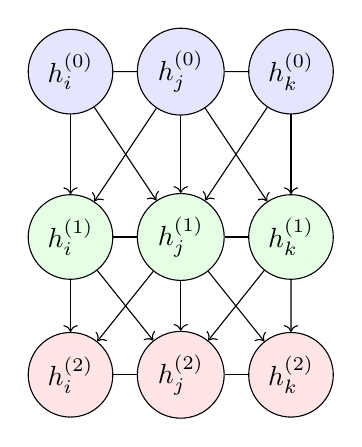
\begin{tikzpicture}[scale=0.7]
                % Layer 0
                \node[circle, draw, fill=blue!10] (A0) at (0,3) {$h_i^{(0)}$};
                \node[circle, draw, fill=blue!10] (B0) at (2,3) {$h_j^{(0)}$};
                \node[circle, draw, fill=blue!10] (C0) at (4,3) {$h_k^{(0)}$};
                
                % Layer 1
                \node[circle, draw, fill=green!10] (A1) at (0,0) {$h_i^{(1)}$};
                \node[circle, draw, fill=green!10] (B1) at (2,0) {$h_j^{(1)}$};
                \node[circle, draw, fill=green!10] (C1) at (4,0) {$h_k^{(1)}$};
                
                % Layer 2
                \node[circle, draw, fill=red!10] (A2) at (0,-2.5) {$h_i^{(2)}$};
                \node[circle, draw, fill=red!10] (B2) at (2,-2.5) {$h_j^{(2)}$};
                \node[circle, draw, fill=red!10] (C2) at (4,-2.5) {$h_k^{(2)}$};
                
                % Connect nodes within layers
                \draw (A0) -- (B0) -- (C0);
                \draw (A1) -- (B1) -- (C1);
                \draw (A2) -- (B2) -- (C2);
                
                % Connect layers
                \draw[->] (A0) -- (A1);
                \draw[->] (B0) -- (A1);
                
                \draw[->] (B0) -- (B1);
                \draw[->] (A0) -- (B1);
                \draw[->] (C0) -- (B1);
                
                \draw[->] (C0) -- (C1);
                \draw[->] (B0) -- (C1);
                
                % Similar arrows for layer 2
                \draw[->] (A1) -- (A2);
                \draw[->] (B1) -- (A2);
                
                \draw[->] (B1) -- (B2);
                \draw[->] (A1) -- (B2);
                \draw[->] (C1) -- (B2);
                
                \draw[->] (C1) -- (C2);
                \draw[->] (B1) -- (C2);
            \end{tikzpicture}
        \end{column}
    \end{columns}
\end{frame}

\begin{frame}[fragile]{Implementing a GCN Layer}
    \begin{lstlisting}[language=Python, basicstyle=\ttfamily\scriptsize]
from torch_geometric.nn import MessagePassing
from torch_geometric.utils import add_self_loops, degree

class GCNConv(MessagePassing):
    def __init__(self, in_channels, out_channels):
        super().__init__(aggr='add')
        self.lin = nn.Linear(in_channels, out_channels)

    def forward(self, x, edge_index):
        # Add self-loops
        edge_index, _ = add_self_loops(edge_index, num_nodes=x.size(0))
        x = self.lin(x)

        # Compute normalization
        row, col = edge_index
        deg = degree(row, x.size(0), dtype=x.dtype)
        deg_inv_sqrt = deg.pow(-0.5)
        norm = deg_inv_sqrt[row] * deg_inv_sqrt[col]

        return self.propagate(edge_index, x=x, norm=norm)

    def message(self, x_j, norm):
        return norm.view(-1, 1) * x_j
    \end{lstlisting}
\end{frame}

\begin{frame}[fragile]{Building a Complete GNN Model}
    \begin{lstlisting}[language=Python, basicstyle=\ttfamily\scriptsize]
class GCN(torch.nn.Module):
    def __init__(self, num_node_features, num_classes):
        super(GCN, self).__init__()
        self.conv1 = GCNConv(num_node_features, 64)
        self.conv2 = GCNConv(64, 64)
        self.conv3 = GCNConv(64, 64)
        self.lin = nn.Linear(64, num_classes)

    def forward(self, data):
        x, edge_index = data.x, data.edge_index

        # Graph Conv layers
        x = F.relu(self.conv1(x, edge_index))
        x = F.dropout(x, p=0.1, training=self.training)

        x = F.relu(self.conv2(x, edge_index))
        x = F.dropout(x, p=0.1, training=self.training)

        x = F.relu(self.conv3(x, edge_index))

        # Global pooling
        x = global_mean_pool(x, data.batch)

        return self.lin(x)
    \end{lstlisting}
\end{frame}

\begin{frame}{Global Pooling: Aggregating Node Features}
    After GCN layers, we need \textbf{one vector per graph} for graph-level predictions:

    \vspace{0.5cm}

    \begin{columns}
        \begin{column}{0.32\textwidth}
            \textbf{Mean Pooling}
            $$h_G = \frac{1}{|V|}\sum_{v \in V} h_v$$

            \vspace{0.2cm}

            \textcolor{accent1}{$\checkmark$} Balanced representation

            \textcolor{warning}{$\times$} Averages out extremes
        \end{column}
        \begin{column}{0.32\textwidth}
            \textbf{Max Pooling}
            $$h_G = \max_{v \in V} h_v$$

            \vspace{0.2cm}

            \textcolor{accent1}{$\checkmark$} Captures key features

            \textcolor{warning}{$\times$} Loses global context
        \end{column}
        \begin{column}{0.32\textwidth}
            \textbf{Sum Pooling}
            $$h_G = \sum_{v \in V} h_v$$

            \vspace{0.2cm}

            \textcolor{accent1}{$\checkmark$} Preserves size info

            \textcolor{warning}{$\times$} Size-dependent
        \end{column}
    \end{columns}

    \vspace{0.5cm}

    \begin{block}{Key Question}
        Which pooling method should you use? It depends on your molecular property!
    \end{block}
\end{frame}
%%%%%%%%%%%%%%%%%%%%%%%%%%%%%%%%%%%%%%%%%%%%%%%%%%%%%%%%%%%%%%%%%%%%%%%%%%%%%%%%%%%%%
\begin{frame}{Pooling Methods: Visual Comparison}
    \textbf{Example}: Small molecular graph with 4 nodes

    \vspace{0.3cm}

    \begin{columns}
        \begin{column}{0.4\textwidth}
            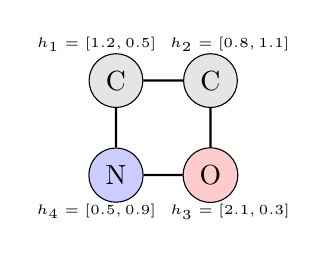
\begin{tikzpicture}[scale=0.8]
                % Molecular graph
                \node[circle, draw, fill=gray!20] (C1) at (0,1.5) {C};
                \node[circle, draw, fill=gray!20] (C2) at (1.5,1.5) {C};
                \node[circle, draw, fill=red!20] (O) at (1.5,0) {O};
                \node[circle, draw, fill=blue!20] (N) at (0,0) {N};

                \draw[thick] (C1) -- (C2) -- (O) -- (N) -- (C1);

                \node[above] at (C1.north west) {\tiny $h_1=[1.2, 0.5]$};
                \node[above] at (C2.north east) {\tiny $h_2=[0.8, 1.1]$};
                \node[below] at (O.south east) {\tiny $h_3=[2.1, 0.3]$};
                \node[below] at (N.south west) {\tiny $h_4=[0.5, 0.9]$};
            \end{tikzpicture}
        \end{column}
        \begin{column}{0.58\textwidth}
            \textbf{After Pooling:}

            \vspace{0.3cm}

            \begin{tabular}{lll}
                \hline
                \textbf{Method} & \textbf{Result} & \textbf{Dim 1, Dim 2} \\
                \hline
                Mean & Average & [1.15, 0.70] \\
                Max & Maximum & [2.1, 1.1] \\
                Sum & Total & [4.6, 2.8] \\
                \hline
            \end{tabular}

            \vspace{0.5cm}

            \textbf{Observations:}
            \begin{itemize}
                \item Mean: Balanced, normalized by size
                \item Max: Captures oxygen's high feature in dim 1
                \item Sum: Keeps magnitude, reflects mol size
            \end{itemize}
        \end{column}
    \end{columns}
\end{frame}
%%%%%%%%%%%%%%%%%%%%%%%%%%%%%%%%%%%%%%%%%%%%%%%%%%%%%%%%%%%%%%%%%%%%%%%%%%%%%%%%%%%%%%%%%%%%%%
\begin{frame}{Experimental Results: ESOL Solubility Dataset}
    \textbf{Question}: Which pooling method works best for predicting water solubility?

    \begin{center}
        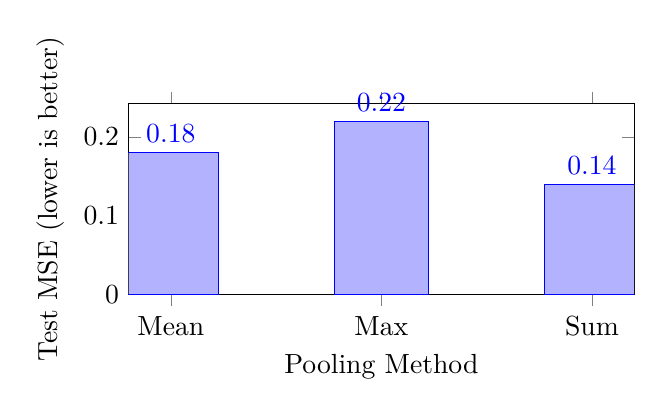
\begin{tikzpicture}
            \begin{axis}[
                ybar,
                symbolic x coords={Mean, Max, Sum},
                xtick=data,
                ylabel={Test MSE (lower is better)},
                xlabel={Pooling Method},
                ymin=0,
                bar width=1.2cm,
                nodes near coords,
                nodes near coords align={vertical},
                legend pos=north east,
                height=4cm,
                width=8cm
            ]
            \addplot coordinates {(Mean,0.18) (Max,0.22) (Sum,0.14)};
            \end{axis}
        \end{tikzpicture}
    \end{center}

    \begin{alertblock}{Result}
        \textbf{Sum pooling wins!} \small Why? Water solubility correlates with molecular size. Larger molecules have more surface area and functional groups affecting solubility.
    \end{alertblock}
\end{frame}
%%%%%%%%%%%%%%%%%%%%%%%%%%%%%%%%%%%%%%%%%%%%%%%%%%%%%%%%%%%%%%%%%%%%%%%%%%%%%%%%%%%%%%%%%
\begin{frame}{When to Use Each Pooling Method}
    \begin{columns}
        \begin{column}{0.48\textwidth}
            \textbf{Mean Pooling}
            \begin{itemize}
                \item \textbf{Best for}: General molecular properties
                \item \textbf{Examples}:
                \begin{itemize}
                    \item Toxicity classification
                    \item LogP (lipophilicity)
                    \item Drug-likeness scores
                \end{itemize}
                \item Size-independent properties
            \end{itemize}

            \vspace{0.2cm}

            \textbf{Max Pooling}
            \begin{itemize}
                \item \textbf{Best for}: Key substructure detection
                \item \textbf{Examples}:
                \begin{itemize}
                    \item Active site identification
                    \item Pharmacophore matching
                    \item Toxicophore detection
                \end{itemize}
                \item Properties dominated by one feature
            \end{itemize}
        \end{column}
        \begin{column}{0.48\textwidth}
            \textbf{Sum Pooling}
            \begin{itemize}
                \item \textbf{Best for}: Size-dependent properties
                \item \textbf{Examples}:
                \begin{itemize}
                    \item Solubility
                    \item Molecular weight prediction
                    \item Molar refractivity
                    \item Surface area estimation
                \end{itemize}
                \item Properties that scale with molecule size
            \end{itemize}

            \vspace{0.5cm}

            \begin{exampleblock}{Pro Tip}
                Try all three and use validation set to choose! Some papers use \textbf{concatenation}: $[h_{mean}, h_{max}, h_{sum}]$
            \end{exampleblock}
        \end{column}
    \end{columns}
\end{frame}
%%%%%%%%%%%%%%%%%%%%%%%%%%%%%%%%%%%%%%%%%%%%%%%%%%%%%%%%%%%%%%%%%%%%%%%%%%%%%%%%%%%%%%%%%%%%%%%
\begin{frame}[fragile]{Loss Function and Optimization}
    \begin{columns}
        \begin{column}{0.45\textwidth}
            \textbf{Common Loss Functions:}
            \begin{itemize}
                \item Binary classification: Binary Cross Entropy
                \item Multi-class: Cross Entropy
                \item Regression: Mean Squared Error
            \end{itemize}
            
            \textbf{Optimization:}
            \begin{itemize}
                \item Adam optimizer is commonly used
                \item Learning rate scheduling can help
                \item Early stopping based on validation
            \end{itemize}
        \end{column}
        \begin{column}{0.55\textwidth}
            \begin{lstlisting}[language=Python, basicstyle=\ttfamily\footnotesize, breaklines=true, breakatwhitespace=true]

# Binary classification
criterion = nn.BCEWithLogitsLoss()

# Regression
criterion = nn.MSELoss()

# Optimizer
optimizer = torch.optim.Adam(
    model.parameters(), 
    lr=0.01,
    weight_decay=5e-4
)

# Learning rate scheduler
scheduler = torch.optim.lr_scheduler.ReduceLROnPlateau(
    optimizer, 
    mode='min', 
    factor=0.5, 
    patience=5
)
            \end{lstlisting}
        \end{column}
    \end{columns}
\end{frame}
%%%%%%%%%%%%%%%%%%%%%%%%%%%%%%%%%%%%%%%%%%%%%%%%%%%%%%%%%%%%%%%%%%%%%%%%%%%%%%%
\begin{frame}[fragile]{Training Loop}
    \begin{lstlisting}[language=Python, basicstyle=\ttfamily\scriptsize]
def train(model, loader, optimizer, criterion):
    model.train()
    total_loss = 0
    for data in loader:
        optimizer.zero_grad()
        out = model(data)
        loss = criterion(out, data.y)
        loss.backward()
        optimizer.step()
        total_loss += loss.item() * data.num_graphs
    return total_loss / len(loader.dataset)

def evaluate(model, loader, criterion):
    model.eval()
    total_loss = 0
    with torch.no_grad():
        for data in loader:
            out = model(data)
            loss = criterion(out, data.y)
            total_loss += loss.item() * data.num_graphs
    return total_loss / len(loader.dataset)

# Training process
for epoch in range(1, 101):
    train_loss = train(model, train_loader, optimizer, criterion)
    val_loss = evaluate(model, val_loader, criterion)
    scheduler.step(val_loss)
    \end{lstlisting}
\end{frame}
%%%%%%%%%%%%%%%%%%%%%%%%%%%%%%%%%%%%%%%%%%%%%%%%%%%%%%%%%%%%%%%%%%%%%%%%%%%%%%%%%%%
\begin{frame}[fragile]{Evaluation on Test Data}
    \begin{columns}
        \begin{column}{0.4\textwidth}
            \small
            \textbf{Evaluation Metrics:}
            \begin{itemize}
                \item Classification: Accuracy, F1-score, AUC-ROC
                \item Regression: RMSE, MAE, R²
            \end{itemize}

            \vspace{0.3cm}

            \textbf{Evaluation Process:}
            \begin{enumerate}
                \item Load the best model
                \item Run predictions on test set
                \item Calculate metrics
            \end{enumerate}
        \end{column}
        \begin{column}{0.6\textwidth}
            \begin{lstlisting}[language=Python, basicstyle=\ttfamily\scriptsize]
from sklearn.metrics import roc_auc_score

# Load best model
model.load_state_dict(
    torch.load('best_model.pt'))

# Evaluate on test set
model.eval()
preds, targets = [], []

with torch.no_grad():
    for data in test_loader:
        pred = torch.sigmoid(model(data))
        preds.append(pred)
        targets.append(data.y)

preds = torch.cat(preds, dim=0).numpy()
targets = torch.cat(targets, dim=0).numpy()

# Calculate AUC-ROC
auc = roc_auc_score(targets, preds)
            \end{lstlisting}
        \end{column}
    \end{columns}
\end{frame}
%%%%%%%%%%%%%%%%%%%%%%%%%%%%%%%%%%%%%%%%%%%%%%%%%%%%%%%%%%%%%%%%%%%%%%%%%%%%%
\begin{frame}{Visualizing Results}
    \begin{columns}
        \begin{column}{0.5\textwidth}
            \centering
            \includegraphics[width=0.95\textwidth]{Figures/loss_curve.png}

            \vspace{0.2cm}
            Loss Curves
        \end{column}
        \begin{column}{0.5\textwidth}
            \centering
            \includegraphics[width=0.95\textwidth]{Figures/pred-vs_actual.png}

            \vspace{0.2cm}
            Prediction vs Actual
        \end{column}
    \end{columns}
\end{frame}

\begin{frame}{The Oversmoothing Problem}
    \textbf{A critical limitation of deep GNNs}

    \vspace{0.5cm}

    \begin{columns}
        \begin{column}{0.52\textwidth}
            \textbf{What is oversmoothing?}
            \begin{itemize}
                \item Node features become increasingly \textcolor{warning}{similar} with network depth
                \item Loss of \textcolor{warning}{discriminative power}
                \item Performance \textcolor{warning}{degrades} after 3-4 layers
            \end{itemize}

            \vspace{0.5cm}

            \textbf{Why does it happen?}
            \begin{itemize}
                \item Repeated neighborhood averaging
                \item Information from distant nodes overwhelms local features
                \item All nodes converge to global average
            \end{itemize}
        \end{column}
        \begin{column}{0.45\textwidth}
            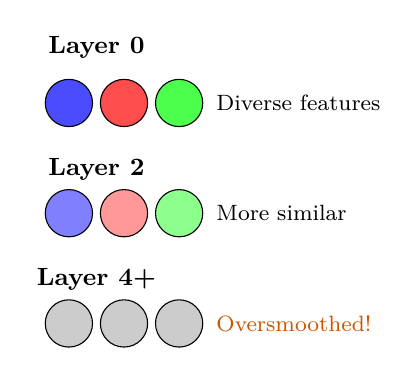
\begin{tikzpicture}[scale=0.7]
                % Layer 0: Diverse features
                \node at (0,5) {\small\textbf{Layer 0}};
                \node[circle, draw, fill=blue!70, minimum size=0.6cm] at (-0.5,4) {};
                \node[circle, draw, fill=red!70, minimum size=0.6cm] at (0.5,4) {};
                \node[circle, draw, fill=green!70, minimum size=0.6cm] at (1.5,4) {};
                \node[right] at (2,4) {\footnotesize Diverse features};

                % Layer 2: More similar
                \node at (0,2.8) {\small\textbf{Layer 2}};
                \node[circle, draw, fill=blue!50, minimum size=0.6cm] at (-0.5,2) {};
                \node[circle, draw, fill=red!40, minimum size=0.6cm] at (0.5,2) {};
                \node[circle, draw, fill=green!45, minimum size=0.6cm] at (1.5,2) {};
                \node[right] at (2,2) {\footnotesize More similar};

                % Layer 4: Nearly identical
                \node at (0,0.8) {\small\textbf{Layer 4+}};
                \node[circle, draw, fill=gray!40, minimum size=0.6cm] at (-0.5,0) {};
                \node[circle, draw, fill=gray!40, minimum size=0.6cm] at (0.5,0) {};
                \node[circle, draw, fill=gray!40, minimum size=0.6cm] at (1.5,0) {};
                \node[right] at (2,0) {\footnotesize \textcolor{warning}{Oversmoothed!}};
            \end{tikzpicture}
        \end{column}
    \end{columns}

    \vspace{0.5cm}

    \begin{alertblock}{Impact}
        Deeper networks don't always mean better performance!
    \end{alertblock}
\end{frame}
%%%%%%%%%%%%%%%%%%%%%%%%%%%%%%%%%%%%%%%%%%%%%%%%%%%%%%%%%%%%%%%%%%%%%%%%%%%%%%%%%%%%
\begin{frame}{Experimental Evidence: Effect of Network Depth}
    \textbf{ESOL solubility prediction}: How does test performance change with depth?

    \begin{center}
        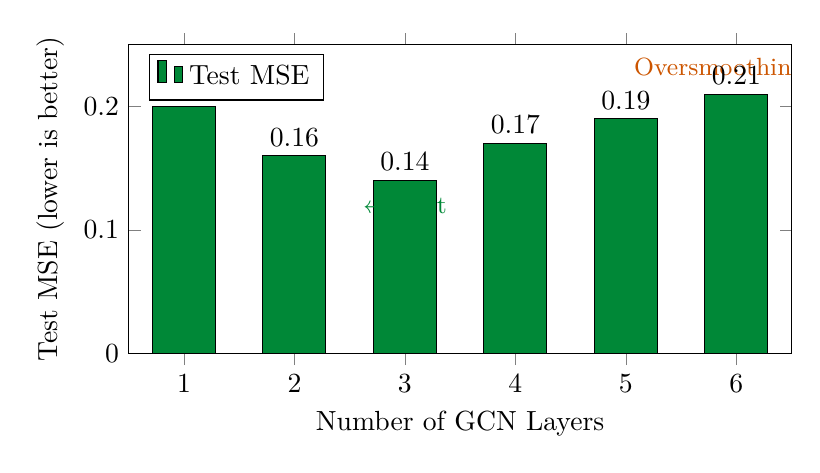
\begin{tikzpicture}
            \begin{axis}[
                ybar,
                symbolic x coords={1, 2, 3, 4, 5, 6},
                xtick=data,
                ylabel={Test MSE (lower is better)},
                xlabel={Number of GCN Layers},
                ymin=0,
                ymax=0.25,
                bar width=0.8cm,
                nodes near coords,
                nodes near coords align={vertical},
                height=5.5cm,
                width=10cm,
                legend pos=north west
            ]
            \addplot[fill=accent1] coordinates {(1,0.20) (2,0.16) (3,0.14) (4,0.17) (5,0.19) (6,0.21)};
            \legend{Test MSE}

            % Add annotation
            \node[draw=none, text=accent1] at (axis cs:3,0.12) {\small ← Best};
            \node[draw=none, text=warning] at (axis cs:6,0.23) {\small Oversmoothing →};
            \end{axis}
        \end{tikzpicture}
    \end{center}

    \begin{exampleblock}{Key Observation}
        \textbf{3 layers} achieve optimal performance. Deeper networks (4-6 layers) perform \textbf{worse} due to oversmoothing.
    \end{exampleblock}
\end{frame}
%%%%%%%%%%%%%%%%%%%%%%%%%%%%%%%%%%%%%%%%%%%%%%%%%%%%%%%%%%%%%%%%%%%%%%%%%%%%%%%%%%%%%%%%%
\begin{frame}{Mathematical Perspective on Oversmoothing}
    \textbf{Why do features converge?}

    \vspace{0.5cm}

    \begin{columns}
        \begin{column}{0.55\textwidth}
            In each GCN layer, node features are averaged:

            $$h_v^{(l+1)} = \sigma\left(\frac{1}{\sqrt{d_v}}\sum_{u \in \mathcal{N}(v)} \frac{h_u^{(l)}}{\sqrt{d_u}} W^{(l)}\right)$$

            \vspace{0.3cm}

            \textbf{After many layers}:
            \begin{itemize}
                \item Each node "sees" exponentially more neighbors
                \item Layer $k$: sees $k$-hop neighborhood
                \item In small molecules, this quickly covers entire graph
                \item Features become weighted average of all nodes
            \end{itemize}
        \end{column}
        \begin{column}{0.42\textwidth}
            \textbf{Feature variance decays}:
            $$\text{Var}(h^{(l)}) \propto \lambda^l$$
            where $\lambda < 1$

            \vspace{0.5cm}

            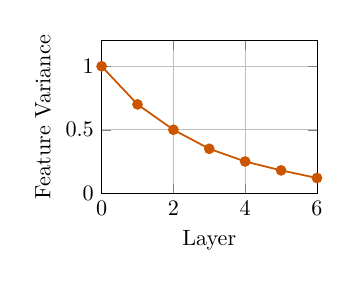
\begin{tikzpicture}[scale=0.8]
                \begin{axis}[
                    xlabel={Layer},
                    ylabel={Feature Variance},
                    xmin=0, xmax=6,
                    ymin=0, ymax=1.2,
                    width=5cm,
                    height=4cm,
                    grid=both
                ]
                \addplot[color=warning, thick, mark=*] coordinates {
                    (0,1.0) (1,0.7) (2,0.5) (3,0.35) (4,0.25) (5,0.18) (6,0.12)
                };
                \end{axis}
            \end{tikzpicture}

            \footnotesize Exponential decay with depth
        \end{column}
    \end{columns}
\end{frame}

\begin{frame}{Chemical Implications of Oversmoothing}
    \begin{columns}
        \begin{column}{0.48\textwidth}
            \textbf{Shallow networks (1-3 layers)}:
            \begin{itemize}
                \item Preserve local chemical environment
                \item Atoms retain distinct features
                \item Can differentiate functional groups
                \item Good for property prediction
            \end{itemize}

            \vspace{0.5cm}

            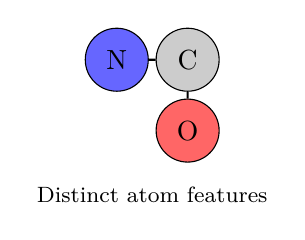
\begin{tikzpicture}[scale=0.6]
                \node[circle, draw, fill=blue!60, minimum size=0.8cm] (N) at (0,1) {N};
                \node[circle, draw, fill=gray!40, minimum size=0.8cm] (C1) at (1.5,1) {C};
                \node[circle, draw, fill=red!60, minimum size=0.8cm] (O) at (1.5,-0.5) {O};

                \draw[thick] (N) -- (C1) -- (O);

                \node[below] at (0.75,-1.5) {\footnotesize Distinct atom features};
            \end{tikzpicture}
        \end{column}
        \begin{column}{0.48\textwidth}
            \textbf{Deep networks (5+ layers)}:
            \begin{itemize}
                \item Atoms become indistinguishable
                \item Loss of local chemical information
                \item Cannot identify reactive sites
                \item Poor discrimination between molecules
            \end{itemize}

            \vspace{0.5cm}

            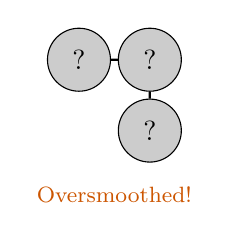
\begin{tikzpicture}[scale=0.6]
                \node[circle, draw, fill=gray!40, minimum size=0.8cm] (N) at (0,1) {?};
                \node[circle, draw, fill=gray!40, minimum size=0.8cm] (C1) at (1.5,1) {?};
                \node[circle, draw, fill=gray!40, minimum size=0.8cm] (O) at (1.5,-0.5) {?};

                \draw[thick] (N) -- (C1) -- (O);

                \node[below] at (0.75,-1.5) {\footnotesize \textcolor{warning}{Oversmoothed!}};
            \end{tikzpicture}
        \end{column}
    \end{columns}

    \begin{block}{The Solution}
        \textbf{Skip connections} (residual learning) allow deeper networks while preserving feature diversity. We'll cover this next!
    \end{block}
\end{frame}
%%%%%%%%%%%%%%%%%%%%%%%%%%%%%%%%%%%%%%%%%%%%%%%%%%%%%%%%%%%%%%%%%%%%%%%%%%%%%%%%%%%%%%
\begin{frame}{Skip Connections: The Solution to Oversmoothing}
    \textbf{Residual Learning for GNNs}

    \vspace{0.5cm}

    \begin{columns}
        \begin{column}{0.52\textwidth}
            \textbf{Key Idea}: Add skip/residual connections

            $$h^{(l+1)} = \text{GCN}(h^{(l)}) + h^{(l)}$$

            \vspace{0.3cm}

            \textbf{Benefits}:
            \begin{itemize}
                \item \textcolor{accent1}{Preserves} information from earlier layers
                \item \textcolor{accent1}{Mitigates} oversmoothing
                \item \textcolor{accent1}{Enables} deeper architectures (5-10+ layers)
                \item \textcolor{accent1}{Improves} gradient flow during training
            \end{itemize}

            \vspace{0.3cm}

            Originally from ResNet (He et al., 2016)\\
            Adapted for GNNs
        \end{column}
        \begin{column}{0.45\textwidth}
            \textbf{Intuition}:
            \begin{itemize}
                \item Identity mapping preserves features
                \item Network learns \textbf{residual} (difference)
                \item Easier to optimize: can always keep identity
                \item Features stay diverse across layers
            \end{itemize}

            \vspace{0.5cm}

            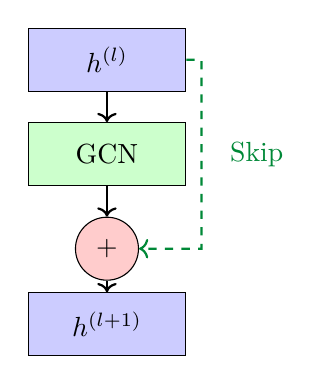
\begin{tikzpicture}[scale=0.8]
                \node[rectangle, draw, fill=blue!20, minimum width=2cm, minimum height=0.8cm] (h0) at (0,3) {$h^{(l)}$};
                \node[rectangle, draw, fill=green!20, minimum width=2cm, minimum height=0.8cm] (gcn) at (0,1.5) {GCN};
                \node[circle, draw, fill=red!20, minimum size=0.8cm] (add) at (0,0) {+};
                \node[rectangle, draw, fill=blue!20, minimum width=2cm, minimum height=0.8cm] (h1) at (0,-1.2) {$h^{(l+1)}$};

                \draw[->, thick] (h0) -- (gcn);
                \draw[->, thick] (gcn) -- (add);
                \draw[->, thick, dashed, accent1] (h0) -- ++(1.5,0) |- (add);
                \draw[->, thick] (add) -- (h1);

                \node[right, accent1] at (1.8,1.5) {Skip};
            \end{tikzpicture}
        \end{column}
    \end{columns}
\end{frame}

\begin{frame}{Architecture Comparison}
    \begin{columns}
        \begin{column}{0.48\textwidth}
            \textbf{Standard GCN}

            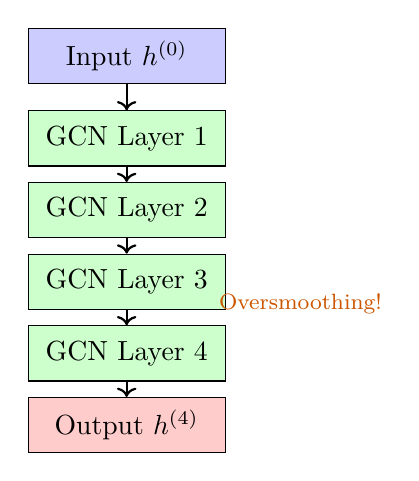
\begin{tikzpicture}[scale=0.7]
                \node[rectangle, draw, fill=blue!20, minimum width=2.5cm, minimum height=0.7cm] (input) at (0,5) {Input $h^{(0)}$};
                \node[rectangle, draw, fill=green!20, minimum width=2.5cm, minimum height=0.7cm] (gcn1) at (0,3.5) {GCN Layer 1};
                \node[rectangle, draw, fill=green!20, minimum width=2.5cm, minimum height=0.7cm] (gcn2) at (0,2.2) {GCN Layer 2};
                \node[rectangle, draw, fill=green!20, minimum width=2.5cm, minimum height=0.7cm] (gcn3) at (0,0.9) {GCN Layer 3};
                \node[rectangle, draw, fill=green!20, minimum width=2.5cm, minimum height=0.7cm] (gcn4) at (0,-0.4) {GCN Layer 4};
                \node[rectangle, draw, fill=red!20, minimum width=2.5cm, minimum height=0.7cm] (output) at (0,-1.7) {Output $h^{(4)}$};

                \draw[->, thick] (input) -- (gcn1);
                \draw[->, thick] (gcn1) -- (gcn2);
                \draw[->, thick] (gcn2) -- (gcn3);
                \draw[->, thick] (gcn3) -- (gcn4);
                \draw[->, thick] (gcn4) -- (output);

                \node[right, warning] at (1.5,0.5) {\footnotesize Oversmoothing!};
            \end{tikzpicture}
        \end{column}
        \begin{column}{0.48\textwidth}
            \textbf{GCN with Skip Connections}

            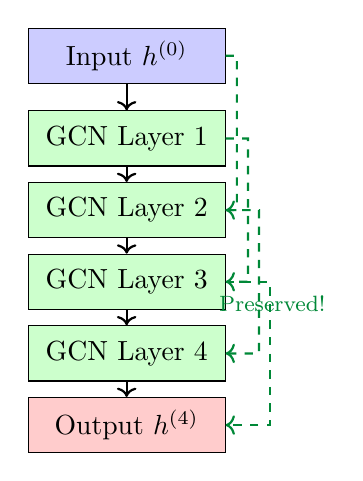
\begin{tikzpicture}[scale=0.7]
                \node[rectangle, draw, fill=blue!20, minimum width=2.5cm, minimum height=0.7cm] (input) at (0,5) {Input $h^{(0)}$};
                \node[rectangle, draw, fill=green!20, minimum width=2.5cm, minimum height=0.7cm] (gcn1) at (0,3.5) {GCN Layer 1};
                \node[rectangle, draw, fill=green!20, minimum width=2.5cm, minimum height=0.7cm] (gcn2) at (0,2.2) {GCN Layer 2};
                \node[rectangle, draw, fill=green!20, minimum width=2.5cm, minimum height=0.7cm] (gcn3) at (0,0.9) {GCN Layer 3};
                \node[rectangle, draw, fill=green!20, minimum width=2.5cm, minimum height=0.7cm] (gcn4) at (0,-0.4) {GCN Layer 4};
                \node[rectangle, draw, fill=red!20, minimum width=2.5cm, minimum height=0.7cm] (output) at (0,-1.7) {Output $h^{(4)}$};

                \draw[->, thick] (input) -- (gcn1);
                \draw[->, thick] (gcn1) -- (gcn2);
                \draw[->, thick] (gcn2) -- (gcn3);
                \draw[->, thick] (gcn3) -- (gcn4);
                \draw[->, thick] (gcn4) -- (output);

                % Skip connections
                \draw[->, thick, dashed, accent1] (input) -- ++(2,0) |- (gcn2);
                \draw[->, thick, dashed, accent1] (gcn1) -- ++(2.2,0) |- (gcn3);
                \draw[->, thick, dashed, accent1] (gcn2) -- ++(2.4,0) |- (gcn4);
                \draw[->, thick, dashed, accent1] (gcn3) -- ++(2.6,0) |- (output);

                \node[right, accent1] at (1.5,0.5) {\footnotesize Preserved!};
            \end{tikzpicture}
        \end{column}
    \end{columns}

    \vspace{0.3cm}

    \begin{block}{Key Difference}
        Skip connections allow information to bypass layers, maintaining feature diversity even in deep networks.
    \end{block}
\end{frame}

\begin{frame}{Experimental Impact: ESOL Dataset}
    \textbf{How much do skip connections help?}

    \vspace{0.1cm}

    \begin{center}
        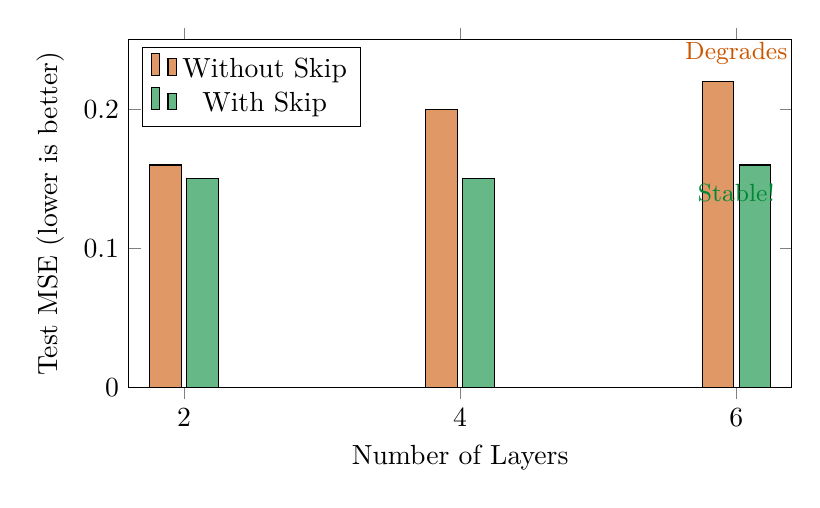
\begin{tikzpicture}
            \begin{axis}[
                ybar,
                bar width=0.4cm,
                ylabel={Test MSE (lower is better)},
                xlabel={Number of Layers},
                symbolic x coords={2, 4, 6},
                xtick=data,
                legend pos=north west,
                ymin=0,
                ymax=0.25,
                width=10cm,
                height=6cm,
                legend style={at={(0.02,0.98)}, anchor=north west}
            ]
            \addplot[fill=warning!60] coordinates {(2,0.16) (4,0.20) (6,0.22)};
            \addplot[fill=accent1!60] coordinates {(2,0.15) (4,0.15) (6,0.16)};
            \legend{Without Skip, With Skip}

            % Annotations
            \node[text=warning] at (axis cs:6,0.24) {\small Degrades};
            \node[text=accent1] at (axis cs:6,0.14) {\small Stable!};
            \end{axis}
        \end{tikzpicture}
    \end{center}

    %\vspace{0.3cm}

    \begin{exampleblock}{Results}
        \begin{itemize}
            \item At \textbf{2 layers}: Skip connections provide \textbf{6\%} improvement
            \item At \textbf{4 layers}: Skip connections provide \textbf{25\%} improvement
            \item At \textbf{6 layers}: Skip connections provide \textbf{27\%} improvement
        \end{itemize}
        \textbf{Conclusion}: More critical for deeper networks!
    \end{exampleblock}
\end{frame}

\begin{frame}[fragile]{Implementation in PyTorch}
    \small
    \textbf{Adding skip connections is straightforward}:

    \begin{columns}
        \begin{column}{0.58\textwidth}
            \begin{lstlisting}[language=Python, basicstyle=\ttfamily\tiny]
class GCNWithSkip(nn.Module):
    def __init__(self, in_channels,
                 hidden_channels,
                 out_channels, num_layers):
        super().__init__()
        self.convs = nn.ModuleList()

        # First layer
        self.convs.append(GCNConv(
            in_channels, hidden_channels))

        # Hidden layers
        for _ in range(num_layers - 2):
            self.convs.append(GCNConv(
                hidden_channels,
                hidden_channels))

        # Output layer
        self.lin = nn.Linear(
            hidden_channels, out_channels)
            \end{lstlisting}
        \end{column}
        \begin{column}{0.4\textwidth}
            \begin{lstlisting}[language=Python, basicstyle=\ttfamily\tiny]
    def forward(self, x,
                edge_index, batch):
        # First layer
        x = F.relu(
            self.convs[0](x, edge_index))

        # Hidden layers with skip
        for conv in self.convs[1:]:
            identity = x  # Save
            x = F.relu(
                conv(x, edge_index))
            x = x + identity  # Skip!

        # Pooling and output
        x = global_mean_pool(x, batch)
        return self.lin(x)
            \end{lstlisting}
        \end{column}
    \end{columns}

    \vspace{0.15cm}

    \begin{alertblock}{Key Lines}
        \footnotesize
        \texttt{identity = x} → Save input; \texttt{x = x + identity} → Add skip connection
    \end{alertblock}
\end{frame}

\begin{frame}{Best Practices and Extensions}
    \small
    \begin{columns}
        \begin{column}{0.48\textwidth}
            \textbf{When to use skip connections}:
            \begin{itemize}
                \item Networks with \textbf{> 3 layers}
                \item When you need deeper representations
                \item Property prediction on large molecules
            \end{itemize}

            \vspace{0.3cm}

            \textbf{Combine with}:
            \begin{itemize}
                \item Batch normalization
                \item Dropout (helps regularization)
                \item Layer normalization
            \end{itemize}
        \end{column}
        \begin{column}{0.48\textwidth}
            \textbf{Advanced variants}:
            \begin{itemize}
                \item \textbf{Dense connections}: Skip from all previous layers

                \item \textbf{Jumping Knowledge (JK) Networks}:
                $$h_{final} = \text{Agg}(h^{(0)}, h^{(1)}, \ldots, h^{(L)})$$

                \item \textbf{Highway connections}: Learn gating
                $$h^{(l+1)} = g \cdot \text{GCN}(h^{(l)}) + (1-g) \cdot h^{(l)}$$
            \end{itemize}
        \end{column}
    \end{columns}

    \vspace{0.3cm}

    \begin{exampleblock}{Recommendation}
        Start simple: Add skip connections to layers 2+. Monitor validation performance to find optimal depth.
    \end{exampleblock}
\end{frame}

\begin{frame}{GNN Advanced Concepts}
    \begin{columns}
        \begin{column}{0.5\textwidth}
            \textbf{Advanced Architectures:}
            \begin{itemize}
                \item GraphSAGE: Scalable inductive representation learning
                \item Graph Attention Networks (GAT): Attention-based message passing
                \item Graph Isomorphism Network (GIN): More powerful than GCN
                \item E(n) Equivariant GNNs: 3D-aware models
            \end{itemize}
        \end{column}
        \begin{column}{0.5\textwidth}
            \textbf{Advanced Techniques:}
            \begin{itemize}
                \item Virtual nodes: Connect all nodes to improve long-range information flow
                \item Edge features: Include bond information
                \item Residual connections: Skip connections in message passing
                \item Graph normalization: Batch norm for graphs
                \item Pre-training: Self-supervised learning on molecules
            \end{itemize}
        \end{column}
    \end{columns}
    
    \vspace{0.5cm}
    
    \begin{center}
        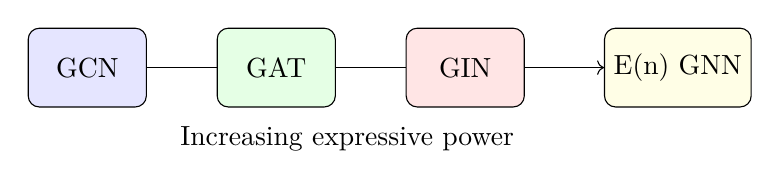
\begin{tikzpicture}[scale=0.6]
            \node[rectangle, draw, fill=blue!10, rounded corners, minimum width=1.5cm, minimum height=1cm] (gcn) at (-1.0,0) {GCN};
            \node[rectangle, draw, fill=green!10, rounded corners, minimum width=1.5cm, minimum height=1cm] (gat) at (3.0,0) {GAT};
            \node[rectangle, draw, fill=red!10, rounded corners, minimum width=1.5cm, minimum height=1cm] (gin) at (7.0,0) {GIN};
            \node[rectangle, draw, fill=yellow!10, rounded corners, minimum width=1.5cm, minimum height=1cm] (en) at (11.5,0) {E(n) GNN};
            
            \draw[->] (gcn) -- (gat) -- (gin) -- (en);
            \node at (4.5,-1.5) {Increasing expressive power};
        \end{tikzpicture}
    \end{center}
\end{frame}

\begin{frame}{Resources and Further Reading}
    \begin{columns}
        \begin{column}{0.5\textwidth}
            \textbf{GitHub Repository:}
            \begin{itemize}
                \item \url{https://github.com/HFooladi/GNNs-For-Chemists}
            \end{itemize}
            
            \textbf{Tutorials:}
            \begin{itemize}
                \item \href{https://distill.pub/2021/gnn-intro/}{"A Gentle Introduction to Graph Neural Networks"}
                \item \href{https://distill.pub/2021/understanding-gnns/}{"Understanding Convolutions on Graphs"}
                \item \href{https://pytorch-geometric.readthedocs.io/en/latest/get_started/introduction.html}{PyTorch Geometric Documentation}
            \end{itemize}
        \end{column}
        \begin{column}{0.5\textwidth}
            \textbf{Research Papers:}
            \begin{itemize}
                \item Kipf \& Welling, "Semi-Supervised Classification with Graph Convolutional Networks"
                \item Gilmer et al., "Neural Message Passing for Quantum Chemistry"
                \item Veličković et al., "Graph Attention Networks"
                \item Xu et al., "How Powerful are Graph Neural Networks?"
            \end{itemize}
        \end{column}
    \end{columns}
    
    \vspace{0.5cm}
    
    \begin{center}
        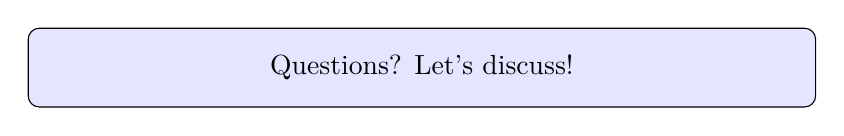
\begin{tikzpicture}
            \node[rectangle, draw, fill=blue!10, rounded corners, minimum width=10cm, minimum height=1cm] at (0,0) {Questions? Let's discuss!};
        \end{tikzpicture}
    \end{center}
\end{frame}

\end{document}